\subsection{Customer Choice Dynamics}
We first show that every customer exhibits the following behavior: until (s)he reaches the phase transition point $i_0(t)$, she visits $A$ only due to the exogeneity paramaeter, and after that (s)he always visits merchant $A$ till she receives the reward.
This behavior is cyclic, and repeats after every reward redemption.

\begin{lemma} $V(i)$ is an increasing function in $i$ if the following condition holds:
\begin{equation}
R > \frac{(1-\lambda)v}{1-\beta}
\end{equation}
And further, $V(i)$ can be evaluated as:
\begin{equation}
V(i) = \max\left\{ \frac{\lambda \beta V(i+1)+(1-\lambda)v}{1-(1-\lambda)\beta}, \beta V(i+1) \right\}
\end{equation}
\end{lemma}

\begin{proof}
First we show that $V(i)$ is an increasing function in $i$ by induction. We first show that if the condition above is satisfied, $V(k-1) < V(k) = R$. Suppose not, so $V(i) \geq R$. Then we have:
\begin{align*}
V(k-1) &= \lambda \beta V(k) + (1-\lambda)(v+\beta V(k-1)) \\
&= \frac{\lambda \beta R + (1-\lambda)v}{1-(1-\lambda)\beta} \\
&< \frac{\lambda \beta R + (1-\beta)R}{1-(1-\lambda)\beta} \\
&= \frac{R(1-(1-\lambda)\beta)}{1-(1-\lambda)\beta} = R
\end{align*}
But this is a contradiction, so $V(k-1) < V(k)$. Now assume $V(i+1) < V(i+2)$ for some $i < k-2$, we will show that this implies $V(i) < V(i+1)$. Suppose not, so $V(i) \geq V(i+1)$. As we did before we may upper bound $V(i)$.
\begin{align*}
V(i) &= \lambda \beta V(i+1) + (1-\lambda)(v+\beta V(i)) \\
&\leq (1-\lambda)v + \beta V(i) \\
\iff V(i) &\leq \frac{(1-\lambda)v}{1-\beta}
\end{align*}
But because $V(i+1) < V(i+2)$, we may lower bound $V(i+1)$.
\begin{align*}
V(i+1) &\geq \lambda \beta V(i+2) + (1-\lambda)(v+\beta V(i+1)) \\
&= (1-\lambda)v + (1-\lambda)\beta V(i+1) + \lambda \beta V(i+2) \\
&> (1-\lambda)+\beta V(i+1) \\
\iff V(i+1) &> \frac{(1-\lambda)v}{1-\beta}
\end{align*}
Again, we have a contradiction, so $V(i) < V(i+1)$, and $V(i)$ is an increasing function in $i$. Now we prove the second claim. We have the following:
\begin{align*}
V(i) &= \lambda \beta V(i+1) + (1-\lambda)\max\{v +\beta V(i), \beta V(i+1) \} \\
&= \max\{\lambda \beta V(i+1) + (1-\lambda)(v+\beta V(i)), \beta V(i+1) \}
\end{align*}

Assuming $V(i)$ is the left term in the above maximum, we may solve the equation for that term.
\begin{gather*}
V(i) = \lambda \beta V(i+1) + (1-\lambda)(v+\beta V(i)) \\
(1-(1-\lambda)\beta) V(i) = \lambda \beta V(i+1) + (1-\lambda)v \\
V(i) = \frac{\lambda \beta V(i+1) + (1-\lambda)v}{1-(1-\lambda)\beta}
\end{gather*}
And we get our claim.
\end{proof}

\begin{theorem} Suppose $V(i)$ is an increasing function in $i$ and consider a customer with look-ahead parameter $t$. A phase transition occurs after (s)he makes $i_0(t)$ visits to firm $A$, where $i_0(t)$ is given by:
\begin{equation}
  i_0(t)=\begin{cases}
    k-\Delta \equiv i_0, & \text{if $t \geq \Delta$}.\\
    k-t, & \text{otherwise}.
  \end{cases}
\end{equation}
with 
\begin{align}
\Delta &= \left\lfloor \log_{\beta}\left(\frac{v}{R(1-\beta)}\right)\right\rfloor
\end{align}
\end{theorem}

\begin{proof}
First we solve for the condition on $V(i+1)$ for us to choose firm $A$ over $B$ willingly.
\begin{gather*}
\beta V(i+1) > \frac{\lambda \beta V(i+1) + (1-\lambda)v}{1-(1-\lambda)\beta} \\
\iff \beta V(i+1) \left(1-\frac{\lambda}{1-(1-\lambda)\beta} \right) > \left(\frac{1-\lambda}{1-(1-\lambda)\beta} \right) v \\
\iff \beta V(i+1) \left(\frac{1-(1-\lambda)\beta -\lambda}{1-(1-\lambda)\beta} \right) > \left(\frac{1-\lambda}{1-(1-\lambda)\beta} \right) v \\
\iff \beta V(i+1) \left(\frac{(1-\lambda)(1-\beta)}{1-(1-\lambda)\beta} \right) > \left(\frac{1-\lambda}{1-(1-\lambda)\beta} \right) v \\
\iff \beta V(i+1) > \frac{v}{1-\beta} \\
\iff V(i+1) > \frac{v}{\beta(1-\beta)}
\end{gather*}
Let $i_0$ be the minimum state $i$ such that the above holds, so in particular $V(i_0) \le \frac{v}{\beta(1-\beta)}$ but $V(i_0+1) > \frac{v}{\beta(1-\beta)}$. We know because $V$ is increasing in $i$, this point is indeed a phase transition: $V(i) > \frac{v}{\beta(1-\beta)}$ for all $i > i_0$, so after this point, the customer always chooses firm $A$. We may compute $V(i_0)$ easily using this fact.
\begin{equation*}
V(i_0) = \beta V(i_0+1) = \cdots = \beta^{k-i_0}V(k) = \beta^{k-i_0}R
\end{equation*}
Thus, we have the following:
\begin{gather*}
\beta^{k-i_0} \le \frac{v}{R\beta(1-\beta)} < \beta^{k-(i_0+1)} \\ 
\iff k-i_0 \ge \log_{\beta}\left(\frac{v}{R\beta(1-\beta)} \right) > k-(i_0+1) \\
\iff i_0 \le k - \log_{\beta}\left(\frac{v}{R(1-\beta)} \right) + 1 < i_0 + 1\\
\iff i_0 = k - \left\lfloor \log_{\beta}\left(\frac{v}{R(1-\beta)}\right) \right\rfloor \equiv k-\Delta
\end{gather*}

The above dependence reduces to the following after incorporating the look-ahead distribution:

\begin{equation*}
  i_0(t)=\begin{cases}
    i_0, & \text{wp } p,\\
    k, & \text{wp } 1-p.
  \end{cases}
\end{equation*}
\end{proof}

Not that the phase transition point is independent of $\lambda$, the customer's visit probability bias toward the merchant.
As we would expect, it increases with the look-ahead parameter, and with the price discount offered by merchant $B$.
And decreases with increase in the reward value $R$ and decrease in the distance to reward $k$.
{\arpit Discussion around what do the $i_0$ dependencies mean.}

{\arpit Discussion around setting $i_0 = 0$}

\subsection{Merchant Objective Dynamics}
We substitute the value of the phase transition point obtained above in the rate of revenue equations to reevaluate them. 
And since we assume that $\lambda$ and $t$ are drawn indepent of each other, we can separate the expectation terms and evaluate them sequentially, first over $t$, then over $\lambda$. This reduces the rate of revenues as follows:

\begin{align*}
RoR_A =& \underset{\lambda, t}E\left[\frac{k-R}{i_0(t)/\lambda + k - i_0(t)}\right]\\
                                       =& \underset{\lambda}E\left[p\cdot\frac{k-R}{i_0/\lambda + k - i_0} + (1-p)\frac{\lambda(k-R)}{k}\right]\\
                                       =& \underset{\lambda}E\left[p\cdot\frac{\lambda(k-R)}{k\lambda + i_0(1-\lambda)} + (1-p)\frac{\lambda(k-R)}{k}\right]\\
                                       =& p\cdot\frac{k-R}{b(k-i_0)^2}\cdot\left(b(k-i_0) - i_0 \log\left(1 + \frac{b(k-i_0)}{i_0}\right)\right) + (1-p)\frac{b(k-R)}{2k}\\
                                       =& p\cdot\frac{k-R}{b\Delta^2}\cdot\left(b\Delta - (k-\Delta)\log\left(1+\frac{b\Delta}{k-\Delta}\right)\right) + (1-p)\frac{b(k-R)}{2k}\\
                                       =& p\cdot\frac{k-R}{\Delta}\cdot\left(1 - \frac{k-\Delta}{b\Delta}\log\left(1+\frac{b\Delta}{k-\Delta}\right)\right) + (1-p)\frac{b(k-R)}{2k}
\end{align*}

\begin{align*}
RoR_B =& \underset{\lambda, t}E\left[\frac{(i_0(t)\lambda - i_0(t))(1-v)}{i_0(t)/\lambda + k - i_0(t)}\right]\\
                                     =& \underset{\lambda}E\left[p\cdot\frac{(i_0/\lambda - i_0)(1-v)}{i_0/\lambda + k - i_0} + (1-p)\frac{(k/\lambda - k)(1-v)}{k/\lambda}\right]\\
                                     =& \underset{\lambda}E\left[p\cdot\frac{i_0(1-\lambda)(1-v)}{k\lambda + i_0(1-\lambda)} + (1-p)(1-\lambda)(1-v)\right]\\
                                     =& p\cdot\frac{i_0(1-v)}{b(k-i_0)^2}\left(k\log\left(1+\frac{b(k-i_0)}{i_0}\right) - b(k-i_0)\right) + (1-p)(1-\frac{b}{2})(1-v)\\
                                     =& p\cdot\frac{(k-\Delta)(1-v)}{b\Delta^2}\left(k\log\left(1+\frac{b\Delta}{k-\Delta}\right) - b\Delta\right) + (1-p)(1-\frac{b}{2})(1-v)\\
                                     =& p\cdot\frac{(k-\Delta)(1-v)}{\Delta}\left(\frac{k}{b\Delta}\log\left(1+\frac{b\Delta}{k-\Delta}\right) - 1\right) + (1-p)(1-\frac{b}{2})(1-v)\label{eq:rorB_eval}
\end{align*}

\subsubsection{Proportional Promotion Budgeting}
First we look into the case when $A$ sets its reward value $R$ proportional to the product of the distance to the reward $k$ and the discount value $v$ provided by merchant $B$: \ie~ $R = \alpha k v$.
We refer to this case as proportional promotion budgeting.
Note $\alpha$ is a constant here.

\begin{theorem}
Under proportional promotion budgeting, the optimal reward distance that $A$ should set is $k = \frac{e}{\alpha(1-\beta)}$ at all values of $b$ as long as $\beta$ is close to 1.
\end{theorem}
\begin{proof}
Recall the previous expression for $RoR_A$. Maximizing this function is equivalent to maximizing the following:
\begin{align*}
\underset{k}\max\{RoR_A\} \Leftrightarrow & \underset{k} \max\left\{\frac{k}{\Delta}\left(1-\frac{k-\Delta}{b\Delta}\log\left(\frac{k-\Delta(1-b)}{k-\Delta}\right)\right)\right\}
\end{align*}
Now let $\theta = \frac{k}{\Delta}$. Then maximizing the above function is equivalent to maximizing the following function w.r.t. $\theta$. Note that $\theta \geq 1$ because $k \geq \Delta$.
\beq\notag
\underset{k}\max\{RoR_A\} \Leftrightarrow \underset{\theta}\max\{f(\theta)\} \Leftrightarrow \underset{\theta}\max\left\{ \theta \left(1-\frac{\theta-1}{b}\log\left(1 + \frac{b}{\theta-1}\right)\right)\right\} 
\eeq

We will show that $f'(\theta) \leq 0$ for all $\theta$ so maximizing $f$ is equivalent to minimizing $\theta$.

\begin{align*}
f'(\theta) &= \frac{2\theta-1+b}{\theta-1+b} - \frac{2\theta-1}{b} \log \left(1+\frac{b}{\theta-1} \right) \\
&= \frac{2\theta-1}{b}\cdot\left(\left(\frac{2\theta-1+b}{\theta-1+b}\right)\left(\frac{b}{2\theta-1} \right) - \log \left(1+\frac{b}{\theta-1} \right)\right) \\
&= \frac{2\theta-1}{b}\cdot\left(\frac{b}{\theta-1+b}+\frac{b^2}{(2\theta-1)(\theta-1+b)} - \log \left(1+\frac{b}{\theta-1} \right)\right)
\end{align*}

Let $g(b, \theta) = \frac{b}{\theta-1+b}+\frac{b^2}{(2\theta-1)(\theta-1+b)} - \log \left(1+\frac{b}{\theta-1} \right)$. 
In the limit of $b \to 0$, it is easy to see that $f'(\theta) = g(b, \theta) = 0$ for all $\theta$ in the domain. 
We now show that for all $\theta$ in the domain and all $0 < b \leq 1$, $\frac{\partial g(b, \theta)}{\partial b} \leq 0$.

\begin{align*}
\frac{\partial g(b,\theta)}{\partial b} &= \frac{\theta-1}{(\theta-1+b)^2}+\frac{1}{2\theta-1}\cdot \frac{2b(\theta-1+b)-b^2}{(\theta-1+b)^2} -\frac{1}{\theta-1+b} \leq 0 \\
&\iff \theta-1 + \frac{2b(\theta-1+b)-b^2}{2\theta-1} \leq \theta-1+b \\
&\iff \frac{b(2\theta-2+b)}{2\theta-1} \leq b \\
&\iff 2\theta-2+b \leq 2\theta-1 \\
&\iff b \leq 1
\end{align*}

Thus we have shown that for all $\theta$, $g(b,\theta) = 0$ as $b \to 0$ and that for all $\theta$ and $0 < b \leq 1$, $g(b,\theta)$ is decreasing. 
These together mean that for all $\theta$ and $b \in [0,1]$, $g(b,\theta) \leq 0$. 
Which implies that $f'(\theta) \le 0$ for all $\theta$ in the domain.
So to maximize $f$, we need to minimize $\theta$.

Now let's look at the quantity $\theta = \frac{k}{\Delta}$.
\begin{align*}
\frac{k}{\Delta} = \frac{k}{\log_\beta\left(\frac{1}{\alpha k(1-\beta)}\right)} \sim \frac{k(1-\beta)}{\log (\alpha k(1-\beta))} 
\end{align*}
The above approximation relies on $\beta$ close to 1. Now this value is minimized at $k = \frac{e}{\alpha(1-\beta)}$. Therefore, for all $b$, the optimal value for $k$ is given by $\frac{e}{\alpha(1-\beta)}$, the value for which $\frac{k}{\Delta}$ is minimized and takes the value $\frac{e}{\alpha}$. 

\end{proof}

An interesting point to observe in the above proof is that maximizing the revenue objective is equivalent to minimizing $\frac{k}{\Delta}$ or maximizing $\frac{\Delta}{k}$. This quantity $\frac{\Delta}{k}$ is effectively the \emph{zone of influence}, \ie, the ratio of number of visits required for a ``forward-looking'' customer to adopt a reward program and the total distance to the reward.
In short, if the merchant minimizes the \emph{zone of influence}, it maximizes its revenue objective.
Merchants often offer reward currency for free (give some examples of airlines issuing free credit or accelerating rate at which points are issued). We are characterizing the time until which it is most beneficial to offer such accelerations. 
The condition that $\beta$ be close to 1 is not very restrictive, as we expect it to be near 1 in most cases {\nolan (maybe get a citation for this)}. Note that because $k \geq \Delta$, the above also shows $\alpha \leq e$. 
Finally, observe that, we need $R > \frac{(1-\lambda)v}{1-\beta}$ for $V$ to be increasing. 
We meet this condition with proportional budgeting when $k = \frac{e}{\alpha(1-\beta)}$ as $R = \alpha k v = \frac{e v}{1-\beta} \geq \frac{v}{1-\beta} \geq \frac{(1-\lambda)v}{1-\beta}$. 
Also note that if $\alpha$ is $1$, then the value of $k$ corresponds to a cashback percentage between $2$ and $4$ as $\beta$ ranges between $0.95$ and $0.9$.
This value is realistic to what is observed in practice too.

Now we evaluate the expected rate of revenues of each merchant under these conditions of proportional budgeting and optimal $k$.

\begin{align*}
RoR_A =& pk\cdot\frac{1-\alpha v}{\Delta}\cdot\left(1 - \frac{k-\Delta}{b\Delta}\log\left(1+\frac{b\Delta}{k-\Delta}\right)\right) + (1-p)\frac{bk(1-\alpha v)}{2k}\\
      =& (1-\alpha v) \left(p\frac{e}{\alpha}\left(1-\frac{e-\alpha}{b\alpha}\log\left(1+\frac{b\alpha}{e-\alpha}\right)\right) + (1-p)\frac{b}{2}\right)
\end{align*}

\begin{align*}
RoR_B =& p\cdot\frac{(k-\Delta)(1-v)}{\Delta}\left(\frac{k}{b\Delta}\log\left(1+\frac{b\Delta}{k-\Delta}\right) - 1\right) + (1-p)(1-\frac{b}{2})(1-v)\\
      =& (1-v)\left(p\cdot\frac{e-\alpha}{\alpha}\left(\frac{e}{b\alpha}\log\left(1+\frac{b\alpha}{e-\alpha}\right) - 1\right)\right)\\
      =& (1-v)\left(p\frac{e}{\alpha}\left(\frac{e-\alpha}{b\alpha}\log\left(1+\frac{b\alpha}{e-\alpha}\right) - \frac{e-\alpha}{e}\right) + (1-p)(1-\frac{b}{2})\right)
\end{align*}

Observe that both the above equations have a left term and a right term. The left term is the rate of revenue obtained from ``forward-looking'' customers whereas the right term is from the myopic customers.
As $\alpha$ ranges between $0$ and $e$, the value on the left term increases from $0$ for $RoR_A$ and decreases to $0$ for $RoR_B$.
That is by controlling the reward budget ratio, merchant $A$ is able to gain the entire ``forward-looking'' customer base.
The next figure illustrates the gap in rate of revenue ($RoR_A - RoR_B$) as follows: for different values of $\alpha$ we plot the region of $b$ and $p$ pairs where the gap is positive.
We observe that there is a clear threshold of $b$ and $p$ beyond which the revenue gap is always positive.
This is easily explained by the increasing nature of the revenue gap with $b$ and $p$.
But more interestingly, the threshold value of $b$ and $p$ decreases as $\alpha$ is increased toward $e$.

\begin{figure*}[t!]
\centering
\begin{subfigure}[t]{0.5\textwidth}
\centering
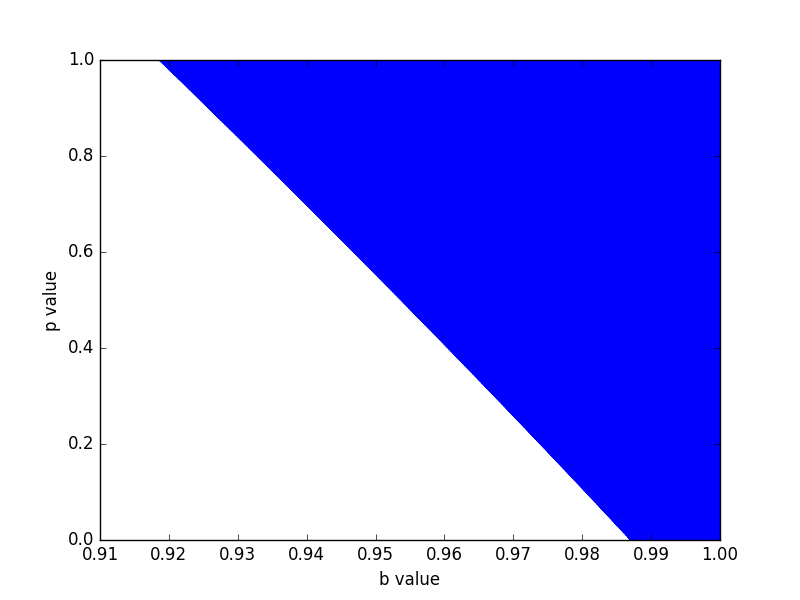
\includegraphics[height=2in]{./figures/bp_pair_rorAB_al0p5_dense.png}
\caption{$\alpha = 0.5$}
\end{subfigure}%
~ 
\begin{subfigure}[t]{0.5\textwidth}
\centering
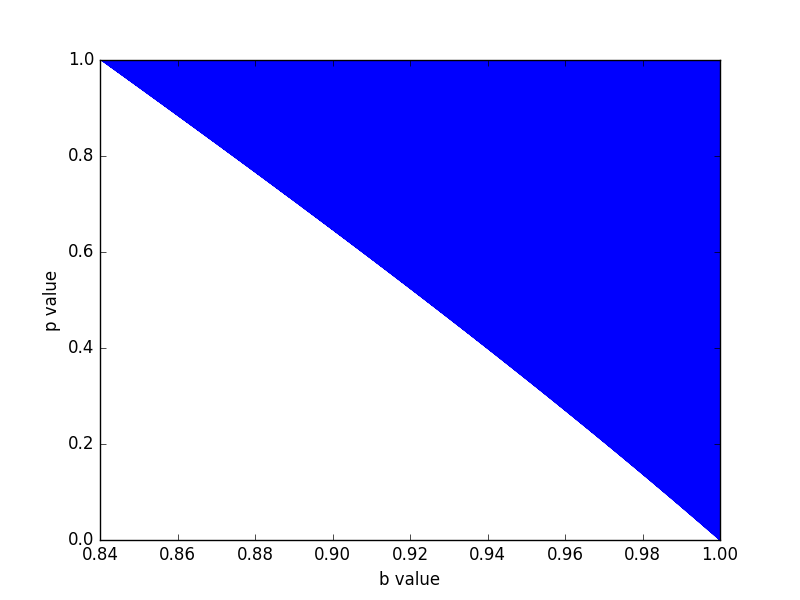
\includegraphics[height=2in]{./figures/bp_pair_rorAB_al1p0_dense.png}
\caption{$\alpha = 1$}
\end{subfigure}
\centering
\begin{subfigure}[t]{0.5\textwidth}
\centering
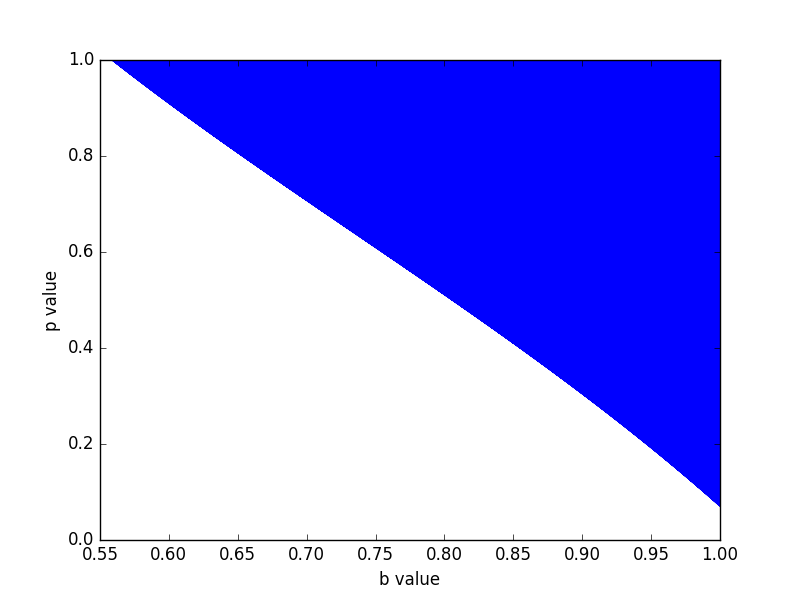
\includegraphics[height=2in]{./figures/bp_pair_rorAB_al2p0_dense.png}
\caption{$\alpha = 2$}
\end{subfigure}%
~ 
\begin{subfigure}[t]{0.5\textwidth}
\centering
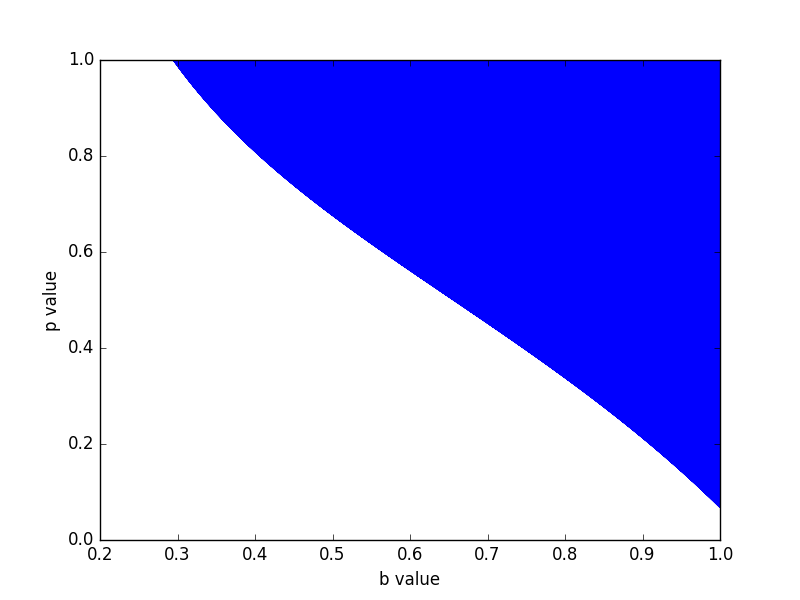
\includegraphics[height=2in]{./figures/bp_pair_rorAB_al2p5_dense.png}
\caption{$\alpha = 2.5$}
\end{subfigure}

\caption{Achievable region of $(b,p)$ pairs where rate of revenue is higher for merchant $A$ for different values of budget proportions $\alpha$. This achievable region is maximized at $\alpha$ close to $e$.}
\end{figure*}

As $\alpha \to 0$, $RoR_A \to (1-p)b/2$, \ie, the revenue earned is only due to visit probability bias.
Observe how $RoR_A$ varies with $\alpha$.
The marginal revenue term $(1-\alpha v)$ decreases with $\alpha$ as the merchant is giving higher rewards to customers, whereas the market share term increases as the merchant gains more ``forward-looking'' customers with increase in reward budget.
Also note that $\alpha = 0$ is equivalent to the merchant not running any reward program.
We next investigate the question of when it is better for the merchant to offer a reward program as opposed to doing traditional pricing.
That is for what values of $\alpha, b, p, v$ is it appropriate for merchant $A$ to offer a reward program.
In other words, when is the rate of revenue of merchant $A$ greater than its rate of revenue at $\alpha = 0$.

\begin{align*}
 (1-\alpha v) \left(p\frac{e}{\alpha}\left(1-\frac{e-\alpha}{b\alpha}\log\left(1+\frac{b\alpha}{e-\alpha}\right)\right) + (1-p)\frac{b}{2}\right) &>& (1-p)b/2\\
\implies (1-\alpha v)p\frac{e}{\alpha}\left(1-\frac{e-\alpha}{b\alpha}\log\left(1+\frac{b\alpha}{e-\alpha}\right)\right) &>& \alpha v (1-p)b/2\\
\implies (1-\alpha v)p\frac{e}{\alpha}\left(\frac{b\alpha}{2(e-\alpha)} - \frac{b^2\alpha^2}{3(e-\alpha)^2}\right) &>& \alpha v (1-p)b/2\\
\implies (1-\alpha v)\frac{pe}{e-\alpha}\left(\frac{1}{2} - \frac{b\alpha}{3(e-\alpha)}\right) &>& \alpha v (1-p)/2\\
\implies \left(\frac{1}{\alpha v}-1\right)\frac{e}{e-\alpha}\left(\frac{1}{2} - \frac{b\alpha}{3(e-\alpha)}\right) &>&  \frac{1-p}{2p}\\
\end{align*}

From above we get an interesting sufficient cutoff for $b$: $b < 3(e-\alpha)/2$.
LHS is decreasing in $v$ and decreasing in $b$.
RHS is decreasing in $p$.

\begin{comment}
\begin{figure}[h!]
\begin{centering}
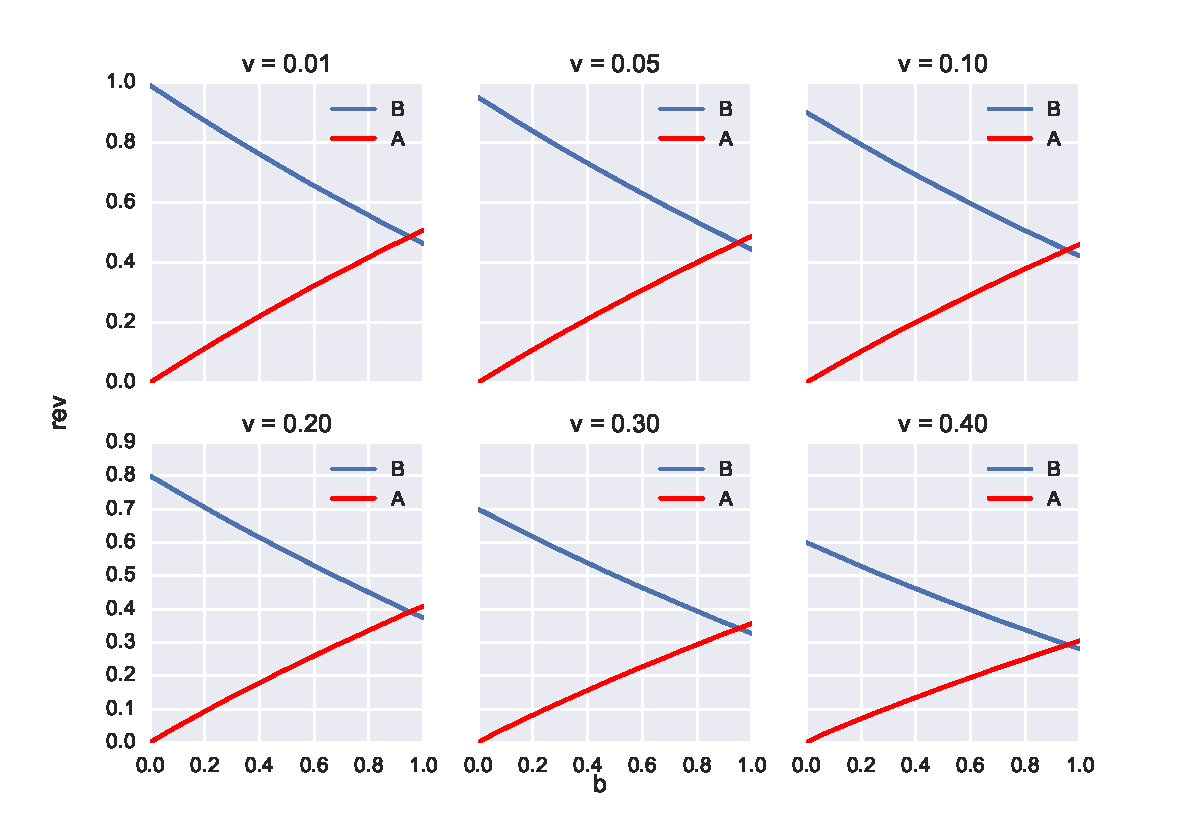
\includegraphics[scale = 0.75]{./figures/eq_budg_vary_v_p05.pdf}
\caption{Rates of revenue for $A$ and $B$ with equal-budgeting as a function of $b$ for various $v$. Fixed $p = 0.5$, $\beta = 0.9$ and $k = e/(1-\beta)$.}
\label{fig:eq_budg_vary_v}
\end{centering}
\end{figure}

Note from the above that $p$, the probability of a consumer being ``forward-looking'' does affect the ratio of expected rates of revenue. Figure~\ref{fig:eq_budg_vary_p} shows simulation results for the rates of revenue of $A$ and $B$ for various values of $p$ with everything else fixed. We see that as $p$ increases, the $b$ required for the reward program to become more profitable than not using one decreases.

\begin{figure}[h!]
\begin{centering}
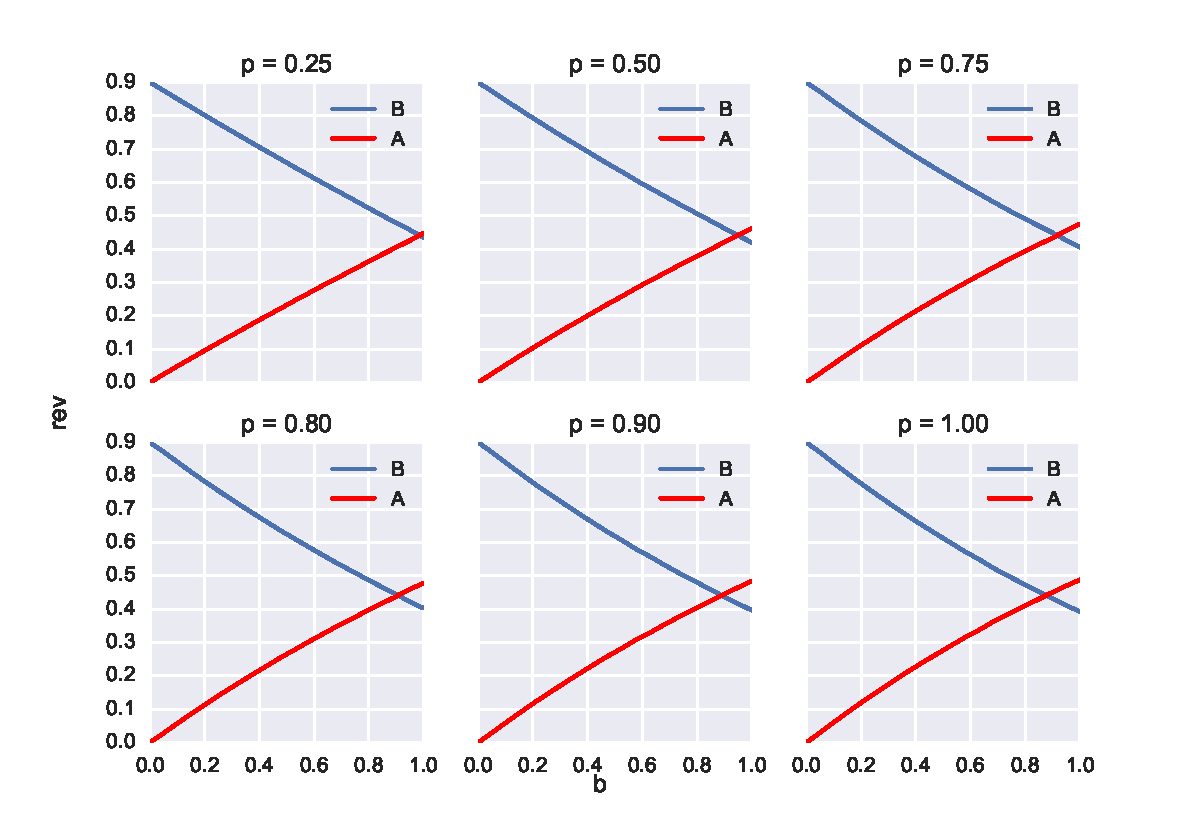
\includegraphics[scale = 0.75]{./figures/eq_budg_vary_p_v01.pdf}
\caption{Rates of revenue for $A$ and $B$ with equal-budgeting as a function of $b$ for various $p$. Fixed $v = 0.1$, $\beta = 0.9$ and $k = e/(1-\beta)$.}
\label{fig:eq_budg_vary_p}
\end{centering}
\end{figure}

{\arpit
\begin{theorem}
When is $RoR_A > RoR_B$ at $i_0 = 0$?
\end{theorem}
}
\end{comment}

{\arpit Talk about the framework in depth. That this can be used to find optimal $R$ and $k$. Also different distributions can be tested once the framework is ready}

\begin{theorem}
Suppose firm $A$ fixes its price at 1, and firm $B$ chooses a price of $1-v$. Given a consumer distribution defined by $p$ - with probability $p$, a consumer is fully forward looking and probability $1-p$ the customer does not look ahead at all - $b$ - each consumer's monopoly factor to firm $A$ is drawn as $\lambda~\sim Unif(0,b)$ and $\beta$ - the customer's discout factor. Then firm $A$ may choose to give a reward of $\alpha v < 1$ to customers after $k$ visits. It should run a reward program if the following condition holds.
\begin{equation}
\frac{1}{b}\left(1-\frac{e-1}{b}\log \left(1+\frac{b}{e-1} \right) \right) \geq \frac{1-(1-p)(1-\alpha v)}{2pe(1-\alpha v)}
\end{equation}
Define the function on the left-hand side above as $g(b)$.
\end{theorem}

\begin{proof}
Firm $A$ always sells the good for price 1. If it chooses to run a reward program its expected rate of revenue is given by:
\begin{equation*}
\underset{\lambda, t}E[RoR_A] = pk(1-\alpha v)\frac{1}{b}\int_0^b \frac{\lambda}{k-(1-\lambda)\Delta} \mbox{ } d\lambda + (1-p)(1-\alpha v)\frac{b}{2}
\end{equation*}
If it does not run a reward program, then the only visits it will receive are exogenous visits. In this case, its expected rate of revenue is simply $\frac{b}{2}$. We consider a reward program to be profitable if its expected rate of revenue is at least that of the non-reward program expected revenue rate.
\begin{gather*}
pk(1-\alpha v)\frac{1}{b}\int_0^b \frac{\lambda}{k-(1-\lambda)\Delta} \mbox{ } d\lambda + (1-p)(1-\alpha v)\frac{b}{2} \geq \frac{b}{2} \\
\iff \frac{pk(1-\alpha v)}{\Delta}\left(1-\frac{k-\Delta}{b\Delta}\log \left(\frac{k-(1-b)\Delta}{k-\Delta} \right) \right) \geq \frac{b}{2}(1-(1-p)(1-\alpha v)) \\
\iff pe(1-\alpha v)\left(1-\frac{e-1}{b}\log \left(1+\frac{b}{e-1} \right) \right) \geq \frac{b}{2}(1-(1-p)(1-\alpha v)) \\
\iff \frac{1}{b}\left(1-\frac{e-1}{b}\log \left(1+\frac{b}{e-1} \right) \right) \geq \frac{1-(1-p)(1-\alpha v)}{2pe(1-\alpha v)}
\end{gather*}
Where we have used the work from Theorem 3.2 as well as the fact that the optimal $k$ is given by $\frac{e}{\alpha(1-\beta)}$, making $\Delta \approx \frac{1}{1-\beta}$. 
\end{proof}

Note that the above condition on $b$ is rather complicated, so we have plotted it as a function of $b$ below. First we notice that $g(b)$ is decreasing in $b$. So for a fixed evaluation of $x \equiv \frac{1-(1-p)(1-\alpha v)}{2pe(1-\alpha v)}$, we are in one of the following cases:
\begin{enumerate}
\item
$x \geq g(0)$. So no value of $b$ makes the reward program profitable.
\item
$x \leq g(1)$. So any value of $b$ makes the reward program profitable.
\item
$x = g(b_0)$ for some $b_0 \in (0,1)$. So the reward program is profitable for all $b \leq b_0$ and not otherwise.
\end{enumerate}

\begin{figure}[h!]
\begin{centering}
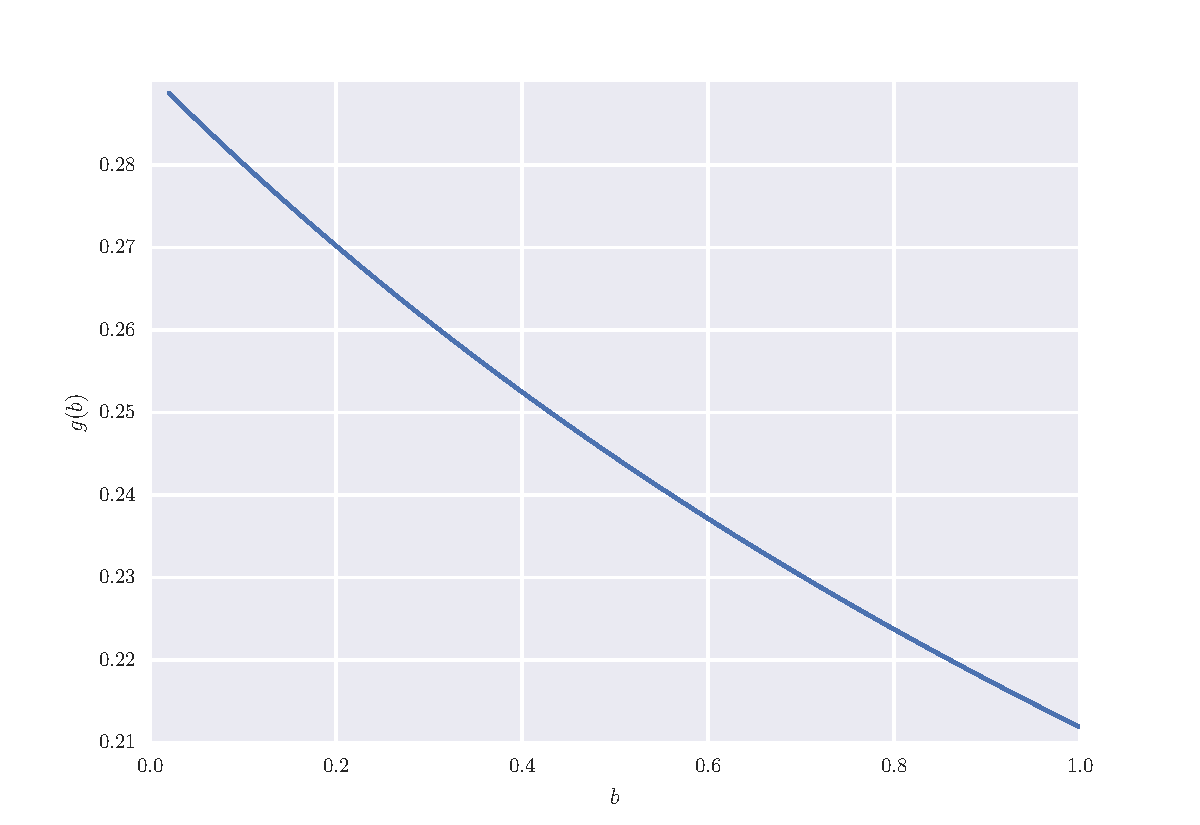
\includegraphics[scale = 0.75]{./figures/b_plot.pdf}
\caption{Function governing profitability of reward program for firm $A$ as a function of $b$.}
\label{fig:b_plot}
\end{centering}
\end{figure}

Now we can take a look at the right hand side of the profitability condition. Let $h(p, \alpha, v) = \frac{1-(1-p)(1-\alpha v)}{2pe(1-\alpha v)}$. It is easy to see that for all values of $p$, $\alpha$ and $v$, $\frac{\partial h}{\partial p} < 0$, $\frac{\partial h}{\partial v} > 0$ and $\frac{\partial h}{\partial \alpha} > 0$. These partial derivative signs mean that as $p$ increases (fixing $v$ and $\alpha$), the interval of profitable $b$'s can only increase. This result make sense intuitively - as the $p$ increases, the number of consumers looking ahead does as well, so more people adopt the reward program. However, increasing either $\alpha$ or $v$ (keeping others fixed), the interval of profitable $b$'s can only decrease. Thus, increasing the reward while keeping $p$ fixed means that in order for the reward program to remain profitable, the profits earned without the reward program must simultaneously decrease, which occurs with decreasing $b$.
